%************************************************
\section{Architecture} % (fold)
\label{sec:architecture}
%************************************************
In this section we will describe the high level components we have developed to accommodate the requirements described in Section \ref{sec:requirements}. To empower the system designer to set up a simulation we need a \emph{Simulation Designer}. Using the simulation designer, the system designer is able to create a \emph{Configured Environment Model}, where all the objects of interest for the simulation have been identified and configured. The \emph{Simulation Runtime} loads a configured environment model and enables the simulation user to control an \emph{Avatar} in order to interact with the environment. As the agent interacts with the environment, the \emph{Context Manager} monitors the agent's position and visual spectrum, delegating the classification of objects around the user to the \emph{SSM Classifier}. The \emph{SSM Sets} can be visualized in the \emph{Context Client} and can be accessed through the \emph{API}.\\

For a better overview, the proposed architecture is illustrated in Figure \ref{fig:initial_architecture}.

\begin{figure}[H]
	\centering
	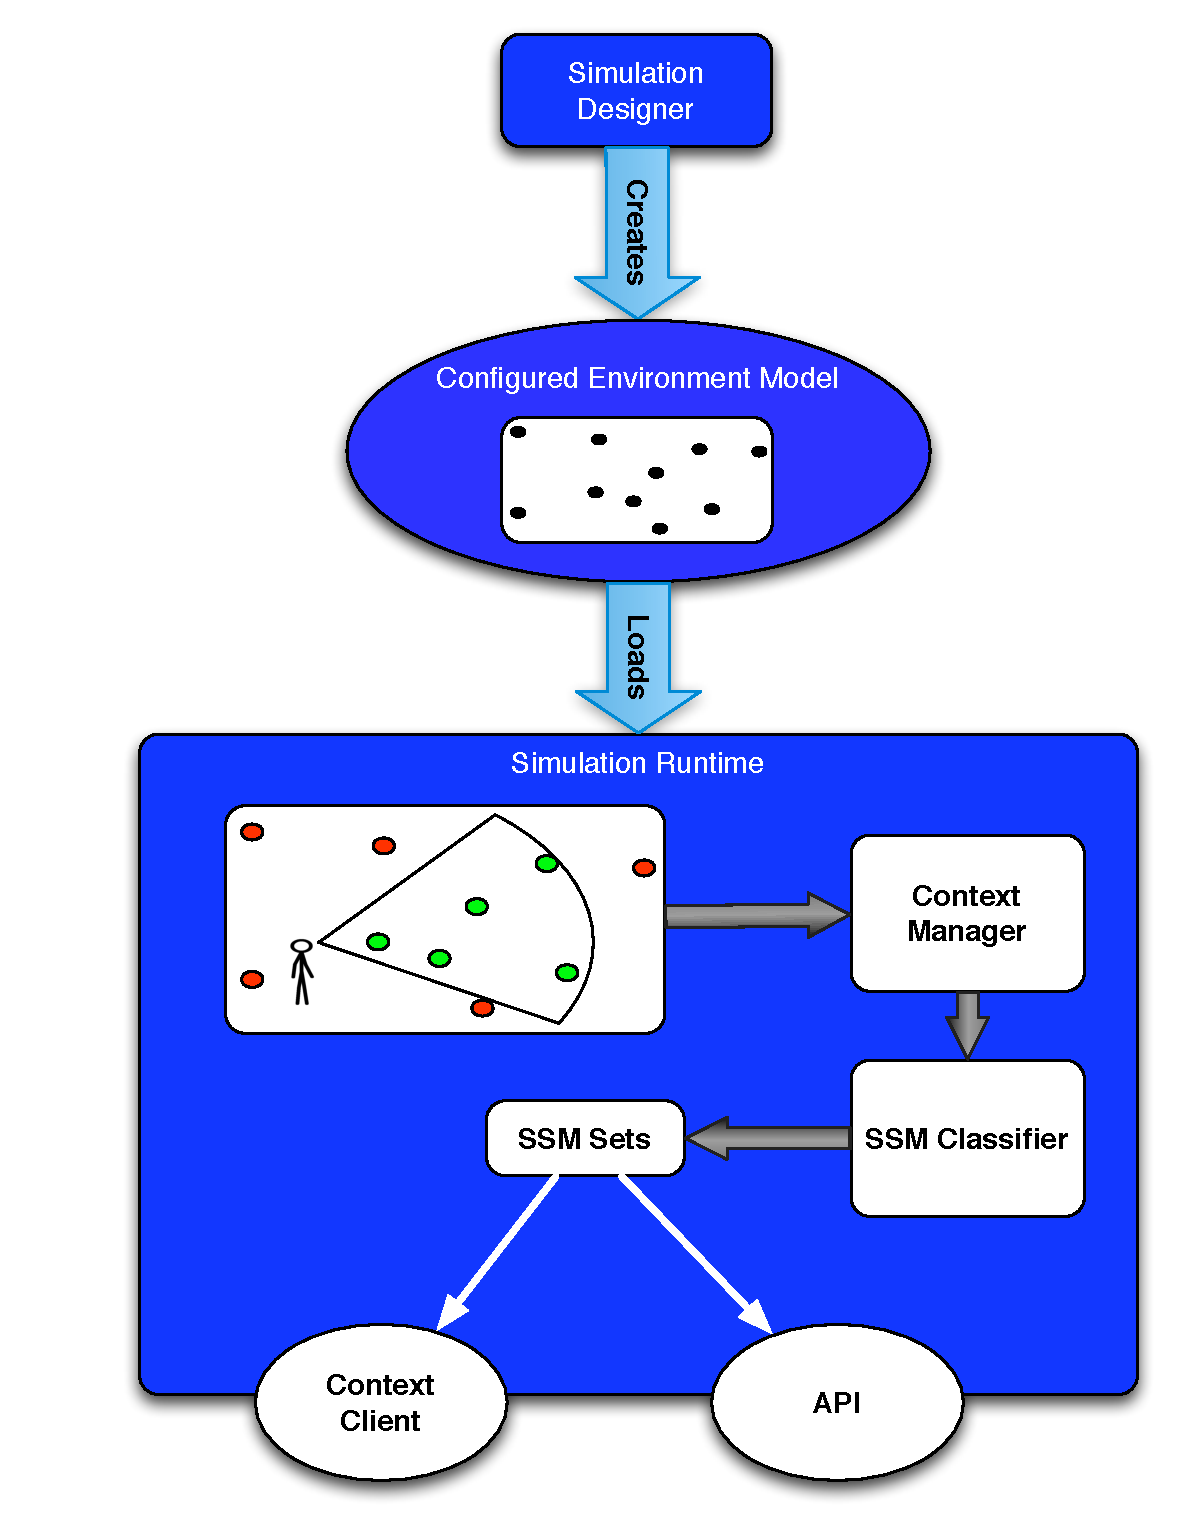
\includegraphics[width=\linewidth]{gfx/Chapter3/initial_architecture}
	\caption{EgoSim Architecture Diagram}
	\label{fig:initial_architecture}
\end{figure}
% Describe the big picture in words and using a picture as well! Describe the main components imposed by this architecture: 3D modelling (to represent the space), rendering and movement control to build the simulated environment, categorization algorithms AND programming API (including the ContextClient).\\

% In the remaining of this chapter good deep into details about why I've chose certain technologies for each component; put each discussion in its own section! To better argue, present several technologies that could fit the same requirements and argue objectively about the the reasons I've made certain choices. I should refer back to arguments in the related work!

% section architecture (end)